\documentclass[12pt]{article}
\usepackage[english]{babel}
\usepackage{apacite}
\usepackage{times}
\usepackage[margin=1in]{geometry}
\usepackage{graphicx} 
\usepackage{float}
\usepackage{amsmath}
\usepackage{booktabs}
\usepackage[svgnames]{xcolor}
\usepackage{xcolor}
\usepackage{listings}
\usepackage{cooltooltips}
\usepackage{colordef}
\usepackage{lvblisting}
\lstset{language=R,
		commentstyle=\color{red}\ttfamily,
		rulecolor=\color{black},
}
\usepackage{subcaption}
\usepackage{setspace}
\lstset{breaklines}
\usepackage{afterpage}
\usepackage[singlelinecheck=false % <-- important
]{caption}
\usepackage[toc,page]{appendix}
\usepackage{fancyhdr}
%\usepackage{hyperref} unfortunatley the package causes several errors in the code, which we were not able to solve, thus the url package is used as an alternative to provide a solution to linking the quantlets.
\usepackage{url}


\pagestyle{fancyplain}

\fancyhf{}

% Quantnet icon (right-aligned)
\newcommand{\quantnet}{\hspace*{\fill} \raisebox{-1pt}{
\includegraphics[scale=0.05]{qletlogo}}\,}

\renewcommand{\footrulewidth}{0pt}
\renewcommand{\headrulewidth}{1pt}
\renewcommand{\sectionmark}[1]{\markboth{#1}{}}
\fancyhead[LE,LO]{\fancyplain{}{\textit{\leftmark}}}
\fancyfoot[CE,CO]{\thepage}

% The following parameters seem to provide a reasonable page setup.
\renewcommand{\baselinestretch}{1.5} 
\topmargin 0.0cm
\oddsidemargin 0.2cm
\textwidth 16,3cm 
\textheight 21cm
\footskip 1.0cm

%%%%%%%%%%%%%%%%% END OF PREAMBLE %%%%%%%%%%%%%%%%




\begin{document} 
\begin{titlepage}
% Double-space the manuscript.

\baselineskip24pt
\title{Statistical Programming Language: \\
How Can The Prediction Of Product Returns Reduce Costs In E-commerce?
}

\author
{Carolin Kunze, Marc-Andre Scheu, Kevin Noessler\\
\\
\normalsize{School of Business and Economics, Humboldt-University of Berlin}\\
}

\date{}
\end{titlepage}
\clearpage\maketitle
\thispagestyle{empty}

%%%%%%%%%%%%%%%%% END OF Title %%%%%%%%%%%%%%%%. 

\newpage
\clearpage
\thispagestyle{empty}

\begin{large}
\textbf{Declaration of Authorship}
\end{large}
\\
\\

We hereby confirm that we have authored this Seminar paper independently and without use
of others than the indicated sources. All passages which are literally or in general matter taken
out of publications or other sources are marked as such.\\

Berlin, 30.03.2018 \quad\quad Carolin Kunze, Marc-Andre Scheu, Kevin Noessler
%%%%%%%%%%%%%%%%% END OF Title %%%%%%%%%%%%%%%%. 

\newpage
\clearpage\maketitle
\thispagestyle{empty}
\tableofcontents

%%%%%%%%%%%%%%%%% END OF Content %%%%%%%%%%%%%%%%. 


\newpage
\setcounter{page}{1}

\section{Introduction}
Product returns represent a substantial challenge in e-commerce which affects the profitability and sustainability of the industry. Approximately 50 percent of all orders are returned and return rates are especially high in the clothing industry \cite{asdecker2015returning}. They cause tremendous costs for online retailers since they are bearing most of the shipping costs. Additional costs result from the item value loss, costs related to processing the return and a higher stock which is needed to compensate the unavailability of an item. Furthermore, product returns severely impact the environment. Nonetheless it isn’t possible to simply deny product returns as a retailer. Apart from the fact that customers have the general right to return products in many countries, free or low-cost shipping has become a standard and customer expectation in the online industry \cite{urbanke2015predicting}. Studies have indeed shown that the return policy affects both purchase rates \cite{wood2001remote} and future buying behavior \cite{petersen2009product}. It is estimated that by lowering the return rates by 10 percent, profitability could increase by over 20 percent \cite{pur2013retourenmanagement}. 


To minimize the costs and increase profitability, it is first necessary to correctly identify orders which are likely to be returned and second to find an appropriate way to cope with these orders. One option is to persuade the customer who is likely to return the product into not buying it by putting a warning sign. The sign could remind the customer of the environmental impact or give recommendations to which size fits best in the clothing industry. Another option is to restrict the payment options so that it is required to pay in advance. The idea behind this is that customers who pay after delivery are twice as likely to return the order \cite{asdecker2015returning}. It is also possible to completely reject the order in extreme cases.

Thus, a targeted intervention including the prediction of product return rates, the identification of orders that are likely to be returned and the prevention of such transactions is remarkably relevant and entails high economic value for the industry. In order to make our predictions as accurate as possible we are going through the four steps of model building, namely feature engineering, model selection, parameter tuning and stacking. However the entire theoretical model building is only useful if companies can actually reduce their costs associated with product returns in practice. Therefore it is necessary to also take the costs into account when building our models, also known as cost-sensitive learning \cite{zadrozny2003cost}. Initially, we will conduct a brief literature review to discuss and evaluate relevant literature for our topic. This shall provide an overview of models that are being used and discover trends in the current literature. We will proceed to explain our methodology, in particular the feature engineering and the models that we use in the machine learning process and explain how we test them. The two main questions how much is the accuracy improving over the model building process and how much can the actual costs be reduced shall be answered. We will figure out and discuss which step of the model building process has the highest effect in terms of accuracy and therefore reduction of costs and which features and models perform best. Furthermore we will assess whether more complex models are worth their effort in building. Finally, we discuss the empirical results and conclude which model provides the best prediction accuracy.

\section{Literature Review}
Product returns have been extensively researched in the literature. Some authors focused on the relevance and identification of the ideal product return policy that balances the costs and benefits. Others examined the impact of return strategies. There are strategies that are focused on the customers e.g. giving product advice and monetary strategies e.g. fee for the shipment costs or discounts for not returning the product. However in comparison to other industries e.g. credit scoring \cite{crook2007recent}\cite{kumar2007bankruptcy} there is very little research in the field of prediction of product returns and the resulting cost reduction. We identified \cite{yu2008hybrid} and \cite{urbanke2015predicting} as most relevant research in the given domain.

Yu and Wang use customers’ demographic data, transaction-based return patterns and product related data to recommend customer and product specific return policies. They base their model on simulated data using Faust’s (1986) survey results \cite{yu2008hybrid}. Urbanke et al. also use an e-commerce data set of product returns. They introduce a new technique for dimension reduction named Mahalanobis Feature Extraction. Yu and Wang’s research is less relevant for e-commerce since their data is not based on real e-commerce transactions. We analyse a very similar data set as Urbanke et al.. However their dataset includes substantially more features. While they reduced dimensionality we add new features to a rather small dimensional data set. In contrast to their introduction of a new machine learning technique we focus on the practical impact of product return predictions.

\section{Methodology}
In this paper the focus is put on the question of how the prediction performance for product returns improves along the model building process and how this prediction can reduce costs. We use several predictive modeling approaches with different underlying classification algorithms to make predictions for our binary target variable $y$, which indicates whether a product was returned ($y$ = 1) or not returned ($y$ = 0) by a customer.
We look at four different tasks within model building: feature engineering, model selection, parameter tuning and as a final step the combination of different model predictions within a meta model, also known as stacking.  \cite{WinNT1}.
Within those steps we compare the prediction performance of five standard machine learning algorithms, decision tree, namely random forest,  logistic regression , regularized logistic regression and neural network. Using these algorithms we train prediction models with the labeled data in order to predict the product returns for the unlabeled data. There are multiple model measurements available to measure prediction performance.
Since we implement five different algorithms and analyse them on several levels of the model building process we decide to only use one performance measure. This makes it easier to evaluate and compare the different results. We use the area under curve (AUC) of the receiver operating characteristics (ROC) as a performance indicator due to its advantage of being independent from a decision threshold and also being an accepted accuracy measure in machine learning. ''The receiver operating characteristics curve compares the classifiers’ performance across the entire range of distributions and error costs'' \cite{ling2003auc}. The receiver operating characteristics curve presents a popular way of visualising classifier performance, finding an appropriate threshold according to the operating condition, thus deriving useful aggregated measures such as the area under the receiver operating characteristics curve \cite{metz1978basic}. The receiver operating characteristics curve presents a popular way of visualising classifier performance, finding an appropriate threshold according to the operating condition, thus deriving useful aggregated measures such as the area under the receiver operating characteristics curve. The area under the curve estimates the probability that a randomly chosen positive is correctly ranked higher than a randomly chosen negative and sumarizes the receiver operating characteristics curve in a single number \cite{metz1978basic}. The more the receiver operating characteristics curve approaches the optimal point, the better are the identified classifier \cite{lessmann2015benchmarking}.


After performing data cleaning on the raw data set we train a rather simple version of the five models which are used as a prediction performance baseline. We refer to them as baseline models throughout our work. While training these models we put moderate effort into creating five to eleven partly distinct features for each model. Additionally we use default parameters where it is required. 
Many machine learning practitioners argue the better the features, the better the results. Even if one does not choose the best models and parameters, one obtains good results by having powerful features that describe the data structure very \cite{WinNT2}. Based on this claim we put a lot of effort into creating a total of 26 input features within four different feature categories. 
As a next step, we train each of the introduced algorithms on the full feature set. While the baseline models can’t be directly compared in terms of algorithm performance because they don’t use the same input features, we can now assess the impact of model selection. Moreover by looking at the area under the curve improvement of the the full feature models in comparison to the baseline models we get an exemplary idea about the human impact on model building through feature engineering. Subsequently, we conduct meta parameter tuning on the more complex models (decision tree, logistic regression, neural networks) to further increase classification accuracy. As a last step, we use stacking to see if a heterogeneous ensemble model can outperform the individual models. 
So far we focused on improving the prediction accuracy of different models. By comparing models based on the area under the curve we do not take costs into account. In order to introduce cost-sensitivity to our model we use empirical thresholding. The technique ``almost always produces the lowest classification cost`` and ``outperforms other cost-sensitive meta-learning methods`` \cite{sheng2006thresholding}.


\section{Experimental Setup}
This section provides a overview of our research implementation. We briefly introduce the data set and explain how we looked at it from different perspectives to create an extensive feature set. We continue to explain the different algorithms tested and how we optimized them through parameter tuning. In order to identify the respective costs, the cost matrix (see Table \ref{tab:cost matrix}) is applied to the model assessment. We finish by explaining the implementation of a second stage stacking model and how we optimized our predictions to minimize costs. 



\subsection{Data}
We work with anonymous real world data of product orders provided by an online fashion retailer. The data has been split into a labeled and an unlabeled dataset with 100,000 and 50,000 observations respectively. Both data sets consist of thirteen input variables. The average return rate of the labeled data set was 48.17 percent , which is about 10 percent lower than the rate observed by  \cite{urbanke2015predicting} . The data contains 27,487 missing and a negligible amount of implausible values. We use common techniques such as imputation with the mean or introducing a new category for implausible or missing values to remove them. Having a closer look at the variables we can tell that the period of collecting data must have been between around 2011 and 2013. Even though we deal with longitudinal data, the split between labeled and unlabeled data set seems to be random. While the unlabeled dataset is used to assess the final model within a competition, we use the labeled dataset for model building and model assessment. Therefore we split it into a training and a test set with 75,000 and 25,000 observations respectively. We create a fold variable for the training set which assigns a random number between one and five to each observation. This will be used for the k-fold method during parameter tuning and stacking.


\subsection{Feature Engineering} \label{subsec:num2}
Feature engineering is the process of extracting more information from existing data by creating new features based on existing variables that make machine learning algorithms work \cite{WinNT3}. 
We use the feature classification suggested by \cite{urbanke2015predicting} 
as a guideline to create relevant features on a customer, a product and a basket level. They considered a similar problem in the paper, yet they were provided with a more extensive feature set. Additionally, we introduce a category of time related variables. This is mainly for practical reasons because four out of thirteen independent variables of the raw data set are dates. Table \ref{tab:features} gives an overview of all created features, their category and the importance measure.
We briefly explain the specifics of feature engineering within the different categories and give an short overview of their importance.
The fact that the labeled and unlabeled data seem to be split randomly, leads to some logic issues when creating features based on customer purchase history or the shopping basket. One might has to use labeled data from the future to make predictions on the past. Yet shopping basket and customer panel data analysis is a common practice in e-commerce \cite{lohse2000consumer}. More importantly, people ordering similar items to have a selection of products to choose from has been described as the main driver of the tremendously high return rates in this industry \cite{asdecker2015returning}. In order to overcome the logical flaw in the raw data we use the independent variables from the unlabeled data set in an unsupervised manner. This allows us to create features like basket size or item duplicates per basket. Our focus on the basket level is to depict similarities of product attributes within a basket. The basic idea is that items with identical or similar item IDs, brands, sizes which are a latent indicator for item categories or colors are substitutable to a certain degree. In order to count such occurrences we create a basket ID based on user ID and order date. 


On a customer level we add age and a dummy variable that indicates whether a person is female, two classical segmentation attributes \cite{anselmsson2006sources} and the total order count as a measure of customer loyalty. 
On the product level the raw data was mostly categorical e.g. item ID, brand ID, item color and item size. The standard way to present categorical data to a machine learning algorithm is dummy coding. This is not an option for several reasons. We compare the performance of different models on the same data set and neural networks need numerical input (see section \ref{sssec:num1}). Furthermore highly dimensional data can lead to further problems in model building and increases computation times. 

\begin{center}
\begin{lstlisting}[frame=single][language=R]
# get factor features
factor_feats = names(tr)[which(unlist(sapply(tr, class)) == "factor")]

# create subset of training set to estimate WOE
set.seed(100)
woe.idx   = createDataPartition(y = tr$return, p = 0.25, list = FALSE)

# decode return level 1 as 'level 1' which will be used as good risk
tr$return = factor(tr$return, levels = c("1", "0"))

# calculate class woes
woe.object = woe(return ~ ., data = tr[woe.idx, ], zeroadj = 0.5)
# change to original format of return
tr$return  = as.integer(as.character(tr$return))

# apply woe to all datasets
datasets = list(class, tr, ts)
ds       = lapply(datasets, function(x) predict(woe.object, newdata = x, replace = T))
\end{lstlisting}
\quantnet {SPLCreateInput} \url{(goo.gl/w5oYkS)}
\end{center}

We therefore use weight of evidence (WoE) \cite{gough2007weight} to transform the categorical and continuous data into numeric features. This assigns a numeric value to each category based on the occurrence rates of the two labels within the given category. 

\begin{center}
	\begin{equation}
WoE= \Big[\ln\Big(\frac{\textnormal{percent of non-events}}{\textnormal{percent of events}}\Big)\Big]
	\end{equation}
\end{center}

Thereby we achieve a reduction in the dimensionality in our models and an increase in the performance, since each category is assinged a unique Weight of Evidence value \cite{wod1985weight}. To avoid overfitting we use a subsample of 25 percent of the training data. In order to be able to calculate the weight of evidence we need to ensure that this subsample contains at least one realization of each label per category. Therefore we assign the least frequent categories to more frequent ones. In order to find similar categories we use a technique known from collaborative filtering \cite{vucetic2000regression}. The general idea is that items or brands which are bought by the same customers are similar. In order to calculate the similarities we create a cross table consisting of user IDs in the rows and category levels in the columns. The cells of the table represent the sum of orders per user and category level. We then calculate the correlation matrix between the different category levels and assign each of the categories lower than a threshold of 100 to the corresponding category with the highest correlation. We then update the similarity table with the reduced categories and repeat this procedure until there is no category left with less realizations than the given threshold. We use a similar approach to cluster colors. Here we use a dictionary \cite{WinNT6} to map RGB (Red-Green-Blue) values to the color names and use the distance instead of customer choices as a similarity measurement.
\begin{center}
\begin{lstlisting}[frame=single][language=R]
brand_clust = function(df, id1 = "user_id", id2 = "brand_id", min_count = 100) {
    # assignes less frequent brands to more frequent ones
    
    df     = df[, c(id1, id2)]
    freq_2 = table(df[, id2])
    # assigne new id to all single occurances
    unique_id2s                         = names(freq_2)[freq_2 == 1]
    df[df[, id2] %in% unique_id2s, id2] = "999999"
    
    # update freq table
    freq_2 = table(df[, id2])
    
    while (min(freq_2) < min_count) {
        # get ids with low frequencies
        low_counts = names(freq_2)[freq_2 < min_count]
        # create cross table of customer ids and brand ids containing order counts
        t             = data.frame(table(df$brand_id, df$user_id))
        names(t)[1:2] = c(id2, id1)
        t_wide        = dcast(t, user_id ~ brand_id)
        # create correlation matrix between brands
        cor = cor(t_wide[, 2:ncol(t_wide)])
        
        #assigne all ids with less than min counts to the id with the highest correlation
        id = low_counts[1]
        for (id in low_counts) {
            # get correlation of ids
            row = cor[id, ][cor[id, ] != 1]
            # assign id to highest correlated category
            assigne_to = names(row[which.max(row)])
            print(paste("assigne: ", id, " to: ", assigne_to))
            df[df[, id2] == id, id2] = assigne_to
        }
        
        freq_2 = table(df[, id2])
        print("min_count:")
        print(min(freq_2))
    }
    # return updated brand ids
    categ = df$brand_id
    return(categ)
}

df$brand_cat = brand_clust(df)

\end{lstlisting}
\quantnet {SPLCreateInput} \url{(goo.gl/w5oYkS)}
\end{center}



Dates contain various time related information, e.g. the day of the month, the week day or the month itself. Moreover, time differences are easy to calculate. We don’t make many assumptions on their relationship towards product returns due to these characteristics. Instead we try to exploit the available information extensively and analyse which relationships emerge. This could be considered a data mining approach \cite{hand2007principles}. The disadvantage of this approach is that it potentially generates highly correlated features and might increase dimensionality with irrelevant features. However we use rather advanced algorithms and don’t expect correlation to have a big impact on model performance \cite{nicodemus2009predictor} adding ten time related variables still results in a fairly small data set.
We deploy Mean Decrease Gini index (MDG) \cite{louppe2013understanding} to assess the influence of single features on class predictions (see Table \ref{tab:features}). Comparing the features with the highest Mean Decrease Gini, item category has the highest impact. Shipment time has a big impact which is interesting for online shops because they are able to influence this variable. The variable time series has the third highest score and represents a simple deterministic time series model based on average daily return rates. The high importance of the feature missing delivery has rather technical implications. There is a perfect correlation between the label zero, e.g. no return and a missing delivery date. The reason for this can be that customers can’t return their orders if they don’t receive them. The top five features are followed by some rather item related features so we can conclude that time and item properties have the largest influence on product returns. Most of the customer features are in the middle of the ranking. It becomes obvious that time variables which are strongly related e.g. Order Day of the Month and the Delivery Day of the Month have very similar importances. This implies a strong correlation. Looking in more detail into this correlation exceeds the scope of this paper, however this seems to be an important topic for subsequent work. 
All features on the basket level are at the end of the importance ranking. Thus, we can’t confirm the claim that ordering multiple items to choose from is a main reason for product returns. This might have to do with specific restrictions of the given online shop or our approach of simply counting co-occurrences of item attributes was too crude. \\

\begin{table}[H]
    \begin{minipage}{.451\linewidth}
      \centering
        \begin{tabular}{lr}
      \hline\hline
      \noalign{\smallskip}
          \textbf{Feature}& \textbf{MDG}\\ 
\hline
\noalign{\smallskip}
\textbf{Time Level}\\ 
Shipment Time & 2234\\
Times Series of daily return rates & 2232 \\
Missing Delivery & 2179\\
Days since Registration & 2123\\
Order Month & 1867\\
Delivery Month & 1814\\
Delivery Day of the Week & 1216\\
Order Day of the Week & 1200\\
Order Day of the Month & 1029\\
Delivery Day of the Month & 1080\\
\noalign{\smallskip}
\noalign{\smallskip}
\textbf{Customer Level} \\ 
Total Customer Orders & 1711\\
State & 1619\\
Age Group & 1380\\
Female  & 143\\
\noalign{\smallskip}
\hline\hline       

        \end{tabular}
    \end{minipage}%
    \begin{minipage}{.5\linewidth}
      \centering
        \begin{tabular}{|lr}
      \hline\hline
      \noalign{\smallskip}
          \textbf{Feature} & \textbf{MDG}\\ 
\hline
\noalign{\smallskip}
\textbf{Product Level} \\ 

Item Category & 2668\\
Item Price & 2071 \\
Total Item Orders & 2037\\
Item Size & 1792\\
Item Color group & 1765\\
Brand Category & 1760\\
Discount at Purchase & 767\\
& \\
& \\

\noalign{\smallskip}
\textbf{Basket Level}\\ 

\noalign{\smallskip}
Basket Size & 992\\
Count of Color Group duplicates & 562\\
Count of Size duplicates & 349\\
Count of Item Category duplicates & 364\\
Count of Brand Category duplicates & 258\\
\noalign{\smallskip}
\hline\hline
        \end{tabular}
    \end{minipage} 
    \vspace{1ex}

     \raggedright    Note: MDG stands for MeanDecreaseGini    
    \caption{Overview of features}
	\label{tab:features}
\end{table}

\newpage
\subsection{Predictive Models}
In the stage of developing predictive models, we build five models with different underlying classification algorithms and conduct parameter tuning. The algorithms decision tree, random forest, logistic regression, regularized logistic regressin and neural networks and our implementation are introduced hereafter.

\subsubsection{Neural Network and Logistic Regression} \label{sssec:num1}
As Tu stated in his research paper \cite{tu1996advantages} in which he compared using logistic regression versus an artificial neural networks to predict medical outcomes both modeling approaches are very similar in their statistical technique. In fact, a "logistic regression model is identical to a neural network model with no hidden layer". The main effect of a neural network versus logistic regression represents the hidden layer where "the network is able to learn [...] complex nonlinear relationship[s] between the dependent and independent variables" \cite{tu1996advantages}. For predicting our target variable $y$ we try both modeling approaches since Tu also concludes that the advantages and disadvantages of both models vary given different data sets and goals \cite{tu1996advantages}.

A neural network consists of an input layer, an output layer and one or multiple hidden layers. In the example below there is shown a very simple neural network with one neuron in the hidden layer.

\begin{figure}[H]
	\begin{center}
     	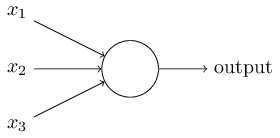
\includegraphics[scale = 0.6]{nn_simple_example.png}
     \end{center}
      \caption{Simple example of a neural network}
           \label{fig:q1}
\end{figure}

\noindent The neural network model has unknwon parameters, often referred to as weights. The weights of the neurons in the hidden layer are initialized randomly, and consist of

\begin{align}
\begin{split}
 \{\gamma_{0m},\gamma_{m}; m=1,2,...,M\} \quad M(p+1)\quad weights,
\\
 \{\kappa_{0k},\kappa_{k}; k=1,2,...,K\} \quad M(p+1)\quad weights.
\end{split}
\end{align}

The complete set of weights is hereafter denoted as $\rho$. For the classification we use either squared error or cross-entropy (deviance):

\begin{center}
	\begin{equation}
  R(\rho)=\sum_{i=1}^n\sum_{k=1}^Ky_ik \log f_k(x_i)
	\end{equation}
\end{center}

The corresponding classifier is provided by \(G(x) = argmax_kf_k(x_i)\). We then feed the neural network with the input variables $x_1, x_2, ...,x_n$ of our training set and their corresponding $y$ labels. While performing backpropagation the weights are getting optimized according to the output error. "The neuron's output, 0 or 1, is determined by whether the weighted sum $\sum_{j}w_jx_j$ is less than or greater than some threshold value" \cite{nielsen2015neural}. The gerneric approach to minimizing \(R(\rho)\) is by gradient descent, refered to as the back-propagation in this setting. The back-propagation for the squared error loss is illustrated in the following equation, with \(z_{mi}=\sigma(\gamma_{0m}+\gamma_m^Tx_i)\) and \(z_i=(z_{1i}, z_{2i},...,z_{Mi})\), we get
	
\begin{eqnarray*}
 R(\rho)& \equiv & \sum_{i=1}^N R_i \\
& =& {} \sum_{i=1}^N\sum_{k=1}^K(y_{ik}-f_k(x_i))^2 \\
\end{eqnarray*}

The derivatives are then 

\begin{align}
\begin{split}
 \frac{\partial R_i}{\partial \kappa_{km}} = -2(y_{ik} - f_k(x_i)) g_k'(\kappa_k^Tz_i)z_mi,
 \\
 \frac{\partial R_i}{\partial \gamma_{ml}} = - \sum_{k=1}^K 2(y_{ik} - f_k(x_i)) g_k'(\kappa_k^Tz_i) \kappa_{km} \sigma '(\gamma_m^Tx_i)x_{il}
\end{split}
\end{align}

In order to train a neural network with our labeled data set, the data should not include any factors and be normalized so that the input variables are in a comparable range. Otherwise some variables may seem to be more important than they actually are \cite{chaturvedi2008soft}. For our neural network we conduct parameter tuning by using cross validation. Cross validation helps us to avoid overfitting. It splits the training data into a smaller training set and a validation set. As we added a column with assigned folds to each data point in our training set, we assure that we train our models with the same training and validation set throughout the training process. We choose to conduct cross validation with five folds. In the code below one can see that we implemented the this by splitting the dataset into an inner training set, containing all folds but the $i$ fold and a validation set consisting of the $i$ fold. Afterwards, we call the training function $do.nn$ for the neural network model. This procedure is used for all the models that we train. 

\begin{center}
\begin{lstlisting}[frame=single][language=R]
k = max(dataset$folds)
for (i in 1:k) {
    # Split data into training and validation by using the folds
    idx.val = which(dataset$folds == i, arr.ind = TRUE)
    cv.train = dataset[-idx.val,]
    cv.val = dataset[idx.val,]
    # call training function for neural network
    do.nn(cv.train, cv.val, i, parameters)
\end{lstlisting}
\quantnet {SPLPredictionNeuralNetworks} \url{(goo.gl/Bj5KnJ)}
\end{center}

This allows to compute performance measurements on data that has not been used during model training. We run a grid search to find the parameter with the highest area under the curve.
Parameter tuning is conducted on the decay which describes the weight decay and is a regularization technique \cite{nielsen2015neural}. A penalty term is added to the error function to penalize large weights that don’t contribute much to reduce the output error during the backpropagation process \cite{witten2016data}. Furthermore, we try different numbers of nodes in the hidden layer which can be tuned by the parameter size in our model. As Jeff Heaton states, a few rule-of-thumb methods we stick to that "the number of hidden neurons should be between the size of the input layer and the size of the output layer". In our case we have 26 input variables and one output variable. By trying up to fifteen nodes in the hidden layer, we can conclude that the size of four nodes in the hidden layer is optimal. Figure \ref{fig:nn} shows the neural network whereas black lines represent positive weights and grey lines negative weights between layers. The line thickness is proportionate to the relative value of each weight \cite{beck2016neural}. The first layer consists of the input variables labeled with $I1$ to $I26$, the second layer is the hidden layer with its nodes labeled with $H1$ to $H4$ and the last layer represents the output variables, in our case only one binary output labeled $O1$. In addition, there are two more nodes $B1$ and $B2$ which are bias nodes. $B1$ is connected to the hidden layer and $B2$ to the output layer. As a simplification, these bias nodes act like a constant in linear regression and is to overcome problems when the values of input variables are zero \cite{tu1996advantages}. We can observe that the input features missing delivery and brand category are connected by very thick black lines to the hidden layer which means that these are positive and relatively large weights. This is consistent with our findings in \ref{subsec:num2}. As the optimal decay is 0.1 after conducting parameter tuning, we can conclude that the decay must be quite important for our neural network. The weight decay limits the weights in growing too large and thus acts as a constraint \cite{krogh1992simple}. 
The technical implementation for the training and paramater tuning phase is shown in the following R code. As described before, we test for different values of size of the hidden layer and weight decay. Therefore, we conduct a gridsearch, which we store in $nnet.params$ containig all values for the parameters to test. In the function $do.nn$, we loop over those parameters and subsequently call the $predict\_and\_validate$ function to compute the area under the curve which we later store in a dataframe to find out the optimal parameters for our neural network model.

\begin{center}
\begin{lstlisting}[frame=single][language=R]
nnet.params = expand.grid("size" = seq(1, 15, 1), "decay" = c(0.1, 0.01, 0.001)) # grid search
do.nn = function(cv.train, cv.val, i){
  for(n in 1:nrow(nnet.param)){
    neuralnet = nnet(return~., data = cv.train,
                     # maxim number of iterations
                     trace = FALSE, maxit = 200,
                     # the number of nodes in the hidden layer
                     size = nnet.param$size[n], 
                     # decay of the weights
                     decay = nnet.param$decay[n])
    predict_validate_nn(neuralnet, cv.val, n, i)
  }
}
\end{lstlisting}
\quantnet {SPLPredictionNeuralNetworks} \url{(goo.gl/Bj5KnJ)}
\end{center}

As introduced before, we also select the logistic regression model for predicting our target variable product returns. In the research paper evaluated earlier it is recommended to use logistic regression when the main goal is to find relationships between the dependent and independent variables \cite{tu1996advantages}. Also in general, a variety of studies in the medical field use logistic regression when the goal is to predict a dichotomous outcome \cite{yusuff2012breast}. In our case, we look for relations between the dependent binary output variable product returns and the independent input variables. The logit model predicts the probability of output variable $Y = 1$ given the independent features in the row vector $X = x$. 
\begin{center}
	\begin{equation}
		p(Y=1|X=x) = \frac{exp\{\beta^Tx\}}{1+exp\{\beta^Tx\}}
	\end{equation}
\end{center}
To estimate the model parameters $\beta$ the return probability is calculated for each data point in the training set. (See below)
\begin{center}
	\begin{equation}
				p(y_i|x_i;\beta)=\Big(\frac{exp\{\beta^T X_i\}}{1+exp\{\beta^TX_i\}}\Big)^{y_i}\Big(1-\frac{exp\{\beta^T X_i\}}{1+exp\{\beta^TX_i\}}\Big)^{1-y_i}
	\end{equation}
\end{center}
Under the i.i.d. assumption for the single data points the likelihood of the dataset is the product of the single data point probabilities. By taking the log likelihood the gradient can be calculated. Since no closed form solution for the optimal parameters exists, the parameter which maximize the data likelihood can be find by using iterative techniques such as gradient decent.
\begin{center}
	\begin{equation}
\nabla_{\beta}l(\beta)=\sum_{i=1}^nx_i\Big(y_i-\frac{exp\{\beta^T x_i\}}{1+exp\{\beta^Tx_i\}}\Big)
	\end{equation}
\end{center}
By training and fitting our logistic regression model, we already obtain a very good prediction model with an area under the curve result similar to the neural network model. When training a model, some variables may be irrelevant and do not have any relation to the target variable. It may also be the case that even though some predictor variables seem to be insignificant, in fact, this is due to high correlations between the predictor variables and vice versa. Two approaches to perform feature selection by not removing predictor variables from the model but from shrinking the coefficients towards zero are ridge regression and the lasso (least absolute shrinkage and selection operator).  "Ridge regression and lasso perform by trading off a small increase in bias for a large decrease in variance of the predictions, hence they may improve the overall prediction accuracy" \cite{pereira2016logistic}.
These regularized logistic regression models can be obtained by adding a penalty term depending on $\lambda$ to the logistic regression formula. The penalties differ for ridge regression and the lasso \cite{ogutu2012genomic}.
\noindent Ridge Regression: 
\begin{center}
	\begin{equation}
				p(y_i|x_i;\beta)=\Big(\frac{exp\{\beta^T x_i\}}{1+exp\{\beta^Tx_i\}}\Big)^{y_i}\Big(1-\frac{exp\{\beta^T x_i\}}{1+exp\{\beta^Tx_i\}}\Big)^{1-y_i} * \beta^2
	\end{equation}
\end{center}
\noindent The Lasso: \\
Given a linear regression with standardized predictors $x_{ij}$ and centred response values $yi$ for $i$ = 1,2,...,$N$ and $j$ = 1,2,....,$p$, the lasso solves the $l_1$-penalized regression problem of finding
$\beta ={\beta_j}$ in order to minimize the following equation.
\begin{center}
	\begin{equation}
				p(y_i|x_i;\beta)=\Big(\frac{exp\{\beta^T x_i\}}{1+exp\{\beta^Tx_i\}}\Big)^{y_i}\Big(1-\frac{exp\{\beta^T x_i\}}{1+exp\{\beta^Tx_i\}}\Big)^{1-y_i} * |\beta|
	\end{equation}
\end{center}
For the parameter tuning, we tested the values of $\alpha$ to be in the range of 0 and 1, i.e. whether ridge regression ($\alpha$ = 0), lasso ($\alpha$ = 1) or an elastic net model ($\alpha$ is in between 0 and 1) leads to a better prediction accuracy. Furthermore, we test the values for $\lambda$, as it refers to a shrinkage penalty. In ridge regression, the larger $\lambda$ gets the closer to zero the estimates of irrelevant variables will be but they will never be exactly zero. This way, the number of included predictors isn’t reduced in this model. On the contrary, the lasso has the advantage of solving this problem by setting estimates exactly equal to zero \cite{pereira2016logistic}. While tuning the parameters, the best value for $\alpha$ turns out to be the lasso default value of 1. For different values of $\lambda$ the effect on the prediction accuracy is very marginal. Nevertheless, the value of 2 for $\lambda$ is the optimal value and thus has a very small effect on the variables. In our model, this conclusion may underlie the fact that we have already selected significant input variables. Our results can only confirm this hypothesis since the regularized logistic regression model and logistic regression model do not differ much in their prediction accuracies.


\newpage
\subsubsection{Tree Based Models}
Decision trees are a well-established classification method. They have been used extensively to predict direct marketing responses \cite{HAUGHTON199742}. For the purpose of our prediction, we use the underlying routines of recursive partitioning (rpart), provided by Therneau, Atkinson, et al.. The general idea is to build a classification model, using a two-stage procedure, which result in a binary tree. Regarding the structure, the leaves of the tree represent class labels and branches represent conjunctions, which consequently lead to the class labels \cite{therneau1997introduction}. We intend to create a classification tree, as our target variable $y$ is binary and thus can only take discrete values. \\

\textbf{Notation:}
\begin{center}
	\(y=\left\{
                \begin{array}{ll}
                  0 \quad if \quad item \quad is \quad kept\\
                  1 \quad if \quad item \quad is \quad returned\\
                \end{array}
              \right.\)\newline\newline
\begin{table}[H]
\centering
\begin{tabular}{lll}
\(\pi_{i}\)      &  & $i$ = 1, 2, ..., $C$ prior probabilities of each observation                                                                                                                                                                  \\
&&\\
$L(i, j)$ &  & \begin{tabular}[t]{@{}l@{}}$i$ = 1, 2, ..., $C$ Loss matrix for incorrectly classifying an $i$ as a $j$.\\ \(L(i, i) = 0\)\end{tabular}                                                                                               \\
&&\\
$A$       &  & \begin{tabular}[t]{@{}l@{}}represents a node of the tree\\ Further $A$ represents a set of individuals in the sample data,\\ and for future data a classification rule\end{tabular} \\
&&\\
$\tau(x)$     &  & true class of an observation $x$, where $x$ is the vector of predictor variables                                                                                                                                              \\
&&\\
$\tau(A)$     &  & the class assigned to $A$, if $A$ were to be taken as a final node                                                                                                                                                            \\
&&\\

\end{tabular}
\end{table}         

\begin{table}[H]
\centering
\begin{tabular}{lll}

\(ni , nA\) &  & \begin{tabular}[t]{@{}l@{}}number of observations, which belong to class $i$ in the sample, number of\\ observations in node $A$\end{tabular}                                                                                                                                                                                                                                  \\
&&\\
$P(A)$    &  & \begin{tabular}[t]{@{}l@{}}probability of $A$ (for future observations) \\ \(\sum_{i=1}^C
\pi_iP\{x\in A |\tau(x)=i\}\) \\ \(\sum_{i=1}^C
\pi_in_{iA}/n_i\)\end{tabular}                                                                               \\
&&\\
$p(i|A)$  &  & \begin{tabular}[t]{@{}l@{}}$P$\(\{\tau(x) = i |x\in A \}\) (for future observations)\\ 
\(=\pi_iP\{x\in A |\tau(x)=i\}/P\{x\in A\}\)\\ 
\(\approx\pi_i(n_{iA}/n_i)/\sum\pi(n_{iA}/n_i)\)\end{tabular}                                                          \\
&&\\
$R(A)$    &  & \begin{tabular}[t]{@{}l@{}}defines risk of $A$ \\ 
\(\sum_{j=1}^k
P(A_j)R(A_j)\)\\ in which $\tau(A)$ is to be chosen to minimize the risk\end{tabular}                                                                                              \\
        &  &                                                                                                                                                                                                                          
\end{tabular}
\end{table}           
\end{center}

Our dataset consists of n observations from $C$ classes and is heterogeneous, consisting of both values of the target variable. Starting from the root node, which contains all of the data, for every feature, it assesses the best way to split the data into $k$ terminal groups; in which for each of the groups, a predicted class is assigned \cite{therneau1997introduction}. We split a node $A$ into two \(A_{L}\) (left) and \(A_{R}\) (right), with this we get

\begin{center}
	\begin{equation}
P(A_{L}) r(A_{L}) + P(A_{R}) r(A_{R}) \leq P(A)r(A)
	\end{equation}
\end{center}


The obvious way to create a decision tree is to choose the split in which the decrease in risk, $\Delta r$, is maximized. The method uses the impurity of a node, as a measurement. Let the function $f$ be a impurity function and we define the impurity of a node $A$ as

\begin{center}
	\begin{equation}
I(A) = \sum_{i=1}^C
f(p_{iA})
	\end{equation}
\end{center}

The proportion of those in $A$, which belong to class $i$, is illustrated by $p_{iA}$ for future samples. In order to achieve that $A$ is pure, we want to get $I(A) =0$. We therefore can distinguish between two candidates for $f$; the information index \(f(p) = -plog(p)\) and the Gini index \(f(p) = p(1-p)\). We proceed to use split that maximises the impurity reduction 

\begin{center}
	\begin{equation}
	\Delta I = p(A)I(A) − p(A_L)I(A_L) − p(A_R)I(A_R)
	\end{equation}
\end{center}

In this case, the best split refers to the node purity. The purity of the parent node before and the degree of purity after the split are compared to determine the information gain. Then, the feature with the highest information gain is used as the split \cite{abbott2014applied}. The steps are repeated for each branch, as the model uses a recursive-partitioning algorithm until all records after the split belong to the same target variable y or until a stop condition is met. The goal is to achieve the best classification with the minimal number of splits. To further increase the performance of the tree and lower the complexity, thus increasing the predictive power, removing branches that make use of features with low importance is essential and referred to as pruning \cite{safavian1991survey}.

\begin{center}
\begin{lstlisting}[frame=single][language=R]
library(rpart)
library(pROC)
# train decision tree and predict the test set
tree       = rpart(return ~ ., data = train, method = "class")
prediction = predict(tree, newdata = test, type = "prob")

# calculate AUC
auc(test$return, prediction[, 2])
\end{lstlisting}
\quantnet {SPLBaselineModels} \url{(goo.gl/UVJQnF)}
\end{center}

Further, a additionial tree based model is represented by a random forest. It is an ensemble model of multiple decision trees. Since it combines multiple models of the same algorithm, it is a homogeneous ensemble model. In order to create individually distinct decision trees, a random forest introduces randomness on two levels. The first one is based on Bootstrap Sampling (select a bootstrap sample from $S$ where $S^{(i)}$ denotes the $i$th bootstrap) also referred to as Bagging. Each tree is built as a random bootstrap sample from the available training data. As a result, every tree is trained on different data. The second level of randomness is introduced by allowing each tree to use only a random subset of features (randomly select some subset of the features \(f \subseteq F\), where $F$ is the set of features) to split the data on \cite{breiman1996out}. The following pseudocode illustrates how the algorithm for a random forest works:

\begin{table}[H]

\begin{tabular}{l}

\hline\hline
\smallskip
\textbf{Random Forest} - Pseudocode                                                                                                                \\ \hline
\begin{tabular}[c]{@{}l@{}}Precondition: Our training set $S$, features $F$, and number of trees in forest $B$.\end{tabular} \\
1. \quad\textbf{function} RandomForest($S$ , $F$)\\
2.  \quad\quad      \(H	\leftarrow \emptyset\)  \\
3.    \quad\quad     \textbf{for} \(i \in 1,.......,B\) \textbf{do                                                                                                              } \\
4.      \quad\quad\quad        \(S^{(i)}	\leftarrow\) A bootstrap sample from $S$                                                                                                   \\
5.     \quad\quad\quad         \(h_{(i)}	\leftarrow\) RandomizedTreeLearn $(S(i), F)$                                                                                                   \\
6.     \quad\quad\quad         \(H	\leftarrow H \cup {h_i}                                                                                                                     \)  \\
7.     \quad\quad      \textbf{end for                                                                                                                               } \\
8.     \quad\quad      \textbf{return $H$                                                                                                                              } \\
9. \quad \textbf{end function                                                                                                                                    } \\
10. \quad \textbf{function} RandomizedTreeLearn$(S , F)$                                                                                                             \\
11.    \quad\quad     At each node:                                                                                                                           \\
12.     \quad\quad\quad          \(f	\leftarrow\) very small subset of $F$                                                                                                        \\
13.      \quad\quad\quad         Split on best feature in $f                                                                                                       $ \\
14.     \quad\quad    \textbf{return} The learned tree                                                                                                                 \\
15. \quad \textbf{end function                                                                                                                                 } \\\hline\hline
\end{tabular}
\caption{Pseudocode Random Forest}
\quantnet {SPLBaselineModels} \url{(goo.gl/UVJQnF)}
\label{my-label}
\end{table}


After building a predefined number of trees the random forest algorithm assigns different weights to the individual trees based on their prediction performance. It is averaged over the weighted tree predictions to calculate its final predictions. The most relevant meta parameter for the random forest is the number of trees which it builds and the size of the allowed feature subset to use for splitting. While the error rate of a random forest generally decreases with the number of trees, it converges. The computing time on the other hand increases linear with the number of trees \cite{breiman2001random}.
Determining the number of trees therefore means to decide which number of trees results in an error rate sufficiently close to the asymptote. Since this is a rather rough estimate we used the Out-of-Bag-Error (OBB-Error) instead of k-folds to determine a good number of trees. This error is calculated on the data that has not been used to built each tree and can therefore be calculated during model building. This avoids time consuming k-folds. To find the right number of trees, we train a random forest with 2500 trees and extract the respective Out-of-Bag-Error given any number of trees.
To remove the high fluctuation between the individual error rates we use a centred moving average of 100. We take the minimal value of the smoothed error rate as a baseline and allow 0.1 percent deviation from it. As Figure \ref{fig:OOB} visulaizes the analysis of the plot, which suggests that 1500 trees provide a sufficient accuracy (see Fig. (\ref{fig:OOB})).

\begin{center}
\begin{lstlisting}[frame=single][language=R]
library(randomForest)
library(forecast)
# load training data
tr = read.csv("../data/base_train3.csv")
# define max number of trees
maxtree  = 2500 
# column indices of non predictors
X_cols   = !(names(tr) %in% c("ID", "folds", "return"))
#train random forest
rf_model = randomForest(tr[, X_cols], factor(tr[, "return"]), ntree = maxtree) 
OOB_err  = rf_model$err.rate[, 1] # get OOB Error

#use moving average of order 100 to smooth OOB Err
ma_full = ma(OOB_err, 100) 

\end{lstlisting}
\quantnet{SPLRandomForestTuning} \url{(goo.gl/L9qrtc)}
\end{center}


 The allowed number of split variables per tree is the second important parameter for random forest training. In order to determine this parameter we use cross validation with 5 folds as described in section \ref{sssec:num1}. We achieve the best area under the curve on the validation sets with two allowed features. One reason for this relatively low count could be that multiple correlated training features could reduced variance between the individual trees. A low number of allowed features per tree might compensate that by increasing the variance.

\begin{figure}[H]
\captionsetup[subfigure]{labelformat=empty}
\centering
\begin{subfigure}{.5\textwidth}
  \centering
  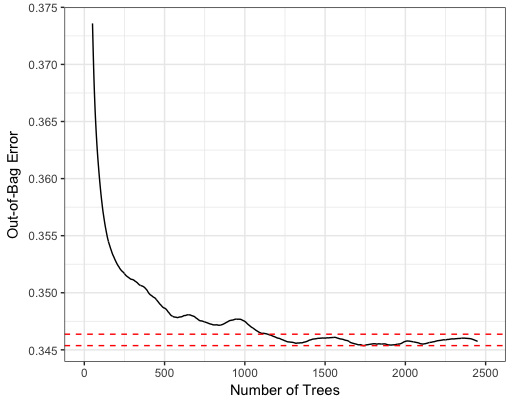
\includegraphics[scale = 0.45]{OBB_Err_ntree.png} 
  \caption{Fig. (2a): Out-of-Bag Error per number of \\trees \quantnet {SPLRandomForestTuning.} \url{(goo.gl/L9qrtc)}}
  \label{fig:OOB}
\end{subfigure}%
\begin{subfigure}{.5\textwidth}
  \centering
  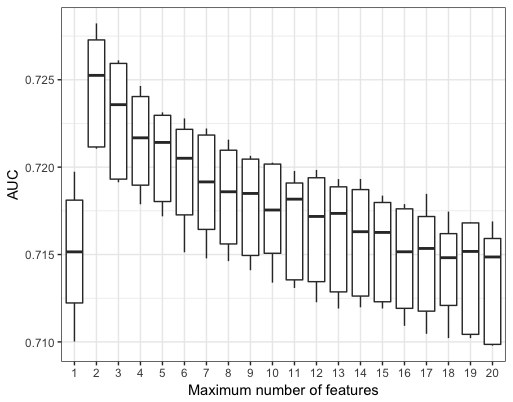
\includegraphics[scale = 0.45]{AUC_mtry.png}
  \caption{Fig. (2b): AUC results over maximal numbers of features \quantnet {SPLRandomForestTuning}} \url{(goo.gl/L9qrtc)}
  \label{fig:AUC}
\end{subfigure}
\label{fig:test}
\end{figure}



\subsection{Stacking and Cost Sensitive Learning}
``Stacking (also called meta ensembling) is a model ensembling technique used to combine information from multiple predictive models to generate a new model." \cite{WinNT5}. In data science competitions, as hosted by www.kaggle.com, such ensemble models have often shown to outperform individual models in prediction accuracy \cite{simidjievski2016modeling}. 
While the prediction improvement is often small considering the increase of model complexity, there are practical reasons for which we decide to use stacking. Firstly, we want to give a comprehensive overview of possible model building tasks and their effects on model performance. Secondly, having a meta model that combines the first stage models, allows us to focus on common performance measurements without worrying about cost optimization during model building. We implement k-folds to create a meta training set that contains the predictions from the first stage models on the training data. In a second step every model is trained on the whole training data set and predictions are performed on the test set. Afterwards, the meta training set is used as input for our second stage model. Since we have already created high complexity a simple logit model is chosen on the second stage. We try several feature combinations from the meta training set. Only a combination of the neural network predictions and the random forest are close to or could improve the area under the curve compared to the random forest as a single model. Whether the area under the curve of the the second stage model is slightly higher or lower depends on the results of the neural network which show some variance over multiple training runs on the same data.
 
While we already include all predictions from the first stage model in the meta train set, it is necessary to run another cross fold validation to predict the product returns with the second stage model. We create a function that calculates the expected costs of product returns based on the item price, the predicted return probability and a given threshold (see Table \ref{tab:cost matrix}). This function is employed within a grid search and calculates the costs for every possible threshold on a range from 1 to 99 percent. The threshold that minimizes the costs on the training set is taken to create final classifications on the test set. In order to make the results independent from the size of the test set, the average return cost per prediction can be calculated. The meta model results in slightly lower average costs for product returns than the random forest model. 
 
\begin{center}
\begin{lstlisting}[frame=single][language=R]
cost_tr = function(pred.prob, true_y, price, threshold = seq(0, 1, 0.01)) {
    # calculates costs based on false positive and false negaitve counts for every threshold in the vector threshold
    
    cost = vector(length = 0)
    for (tr in threshold) {
        
        # make predictions based on threshold value
        pred.cl = ifelse(pred.prob >= tr, 1, 0)
        FN.idx  = which(pred.cl == 0 & true_y == 1)
        FP.idx  = which(pred.cl == 1 & true_y == 0)
        # calculate costs
        FN.cost = sum(-0.5 * price[FN.idx])
        FP.cost = sum(2.5 * (-3 - 0.1 * price[FP.idx]))
        total   = FN.cost + FP.cost
        cost    = c(cost, total)
    }
    cost
}

# calculate training set cost matrix for all models and thresolds on a range from [0,1]
threshold = seq(0, 1, 0.01)
costs     = apply(cbind(tr_meta[, models], meta_tr_yhats), 2, cost_tr, true_y = tr_meta$return, 
    price = tr_meta$item_price, threshold = threshold)

# returns lowest costs per model
apply(costs, 2, max)
# returns threshold in % for lowest cost
opt_th = apply(costs, 2, which.max)

\end{lstlisting}
\quantnet {SPLStacking} \url{(goo.gl/sUXr4M)}
\end{center} 
 
 
\section{Empirical Results}
The graph shown in Figure \ref{fig:AUC result overview} makes it obvious that the biggest area under the curve uplift is achieved through feature engineering. The baseline models which were trained using relatively little programming effort already increase the area under the curve compared to the naive classifier up to 11.67 percent. For practitioners this implies that they can already create some value with relatively little costs and expertise. The area under the curve values for all models increase almost linear from the naive value over the baseline models to the full feature set. This means that we could approximately double the area under the curve increase through more extensive feature engineering. However the baseline models have on average 8.4 features, while the full feature set contains 26 variables. This implies that the improvement per feature is smaller. This seems intuitive for two reasons. On the one hand, one would expect the marginal predictive power per additional feature to be decreasing. On the other hand, we expect to have some highly correlated features which adds redundant information to the models which can lead to overfitting \cite{WinNT4}. 
In general, we can observe that the more complex models random forest and neural network outperform the simpler models on every stage. For the base models, one reason might be different feature sets for training. An indicator for this is that the gradient of the logistic regression and the regularized logistic regression model slightly increases while it slightly decreases for the random forest model. On the full feature set the strongest model, the random forest, outperforms the weakest one by 5.62 percent, the second weakest model by 2.29 percent. Compared to the other steps this implies a medium importance for model selection. Taking model complexity into account, in practice one might prefer a simpler logistic regression model over the complex random forest model. Looking at the uplift through parameter tuning, one can observe a slight increase of 0.27 percent, 0.47 percent and 0.44 percent for the random forest, regularized logistic regression and neural network respectively. This suggests a rather small overall importance of parameter tuning. It is interesting to note that the more complex regularized logistic regression model is outperformed by the simple logistic regression model before parameter tuning and is only 0.02 percent better afterwards. This could mean that the data set is big enough so that overfitting might not be an issue and adding a penalty term is not necessary. By combining the two strongest models random forest and neural network in a meta model the accuracy barely changes, the combined model performs is even worse by 0.002. However this result varies slightly on multiple training and prediction runs. We observe slight area under the curve improvements within the third decimal place as well.

\begin{center}
\begin{figure}[H]
    \begin{scriptsize}
  \begin{center}
      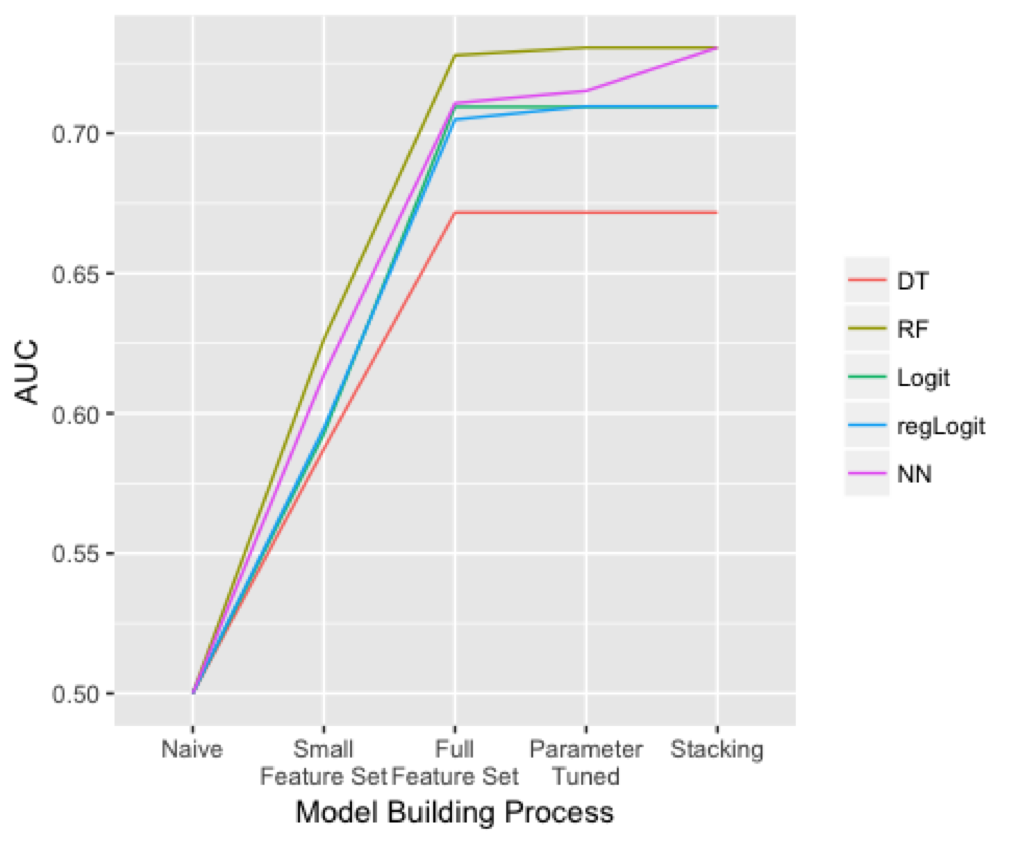
\includegraphics[scale = 0.65]{result_update.png}
      \end{center}
 	\end{scriptsize}
      \begin{center}
    \caption{AUC result overview} 
    \quantnet {SPLStacking} \url{(goo.gl/sUXr4M)}
      \label{fig:AUC result overview}
 		\end{center}
  \end{figure}
\end{center}
 
Looking at the average return costs per order (see Table \ref{table:Average return costs}), the meta model slightly outperforms the random forest. Since the cost reduction is negligible and the change of the area under the curve is not robust, the third stage ensemble model has proven to be irrelevant for model performance while adding unnecessary model complexity. 
Table \ref{table:Average return costs} shows the average cost of product returns per order. It is noticeable that independent from the models we can cut down the costs by half compared to a naive model. These are theoretical values under the assumption that every user who is being influenced not to order, e.g. by showing a warning sign, won’t order. The actual business impact can easily be calculated based on empirical data on customers’ reactions to the warning sign. If we assume that 50 percent change their mind about ordering a certain item, the strongest model can reduce product return costs by around 27 percent. 
\begin{table}[H]
\begin{center}
\begin{tabular}{l|ccccccc} 
\hline\hline
 Algorithm & Naive    &    DT   &     RF   & Logit   &  regLogit  & NN	  &   Stacking \\
\noalign{\smallskip}
\hline
\noalign{\smallskip}
Average return costs & 18.68 & 9.11 & 8.84 & 9.06  & 9.08 & 8.98 & 8.83 \\
\noalign{\smallskip}
\hline\hline
\end{tabular}
\caption{Average return costs.}
\label{table:Average return costs}
\end{center}
\end{table}
\section{Conclusion}
We test various different features and models in the model building process. We find that feature engineering has by far the biggest impact on the model performance. Companies should therefore especially invest in this process. While basket and customer related features only performed moderately well, time and product related features have a major impact on the prediction accuracy. The high importance of shipment time is especially interesting for online retailers since they can directly influence this factor and therefore reduce the return rate and their costs. However, the claim that people order multiple similar items to have a large selection to choose from could not be confirmed. Since this might be due to shop-specific characteristics, we can’t generalize this finding without further information on the data source. Feature interpretation was only a side aspect of our work. However, the results indicate that further research in this field could yield valuable insights. Further importance measurements can be included and a stronger focus on feature correlation and selection can be put. Model selection has a moderate influence on model performance. While more complex models outperformed the simpler models (logistic regression and decision tree) through model building, the performance difference was rather small. It is therefore questionable whether investing in more complex models pays off in practice. This finding is consistent with research in other areas \cite{lessmann2015benchmarking}. Simpler models may be sufficient. Parameter tuning had little impact on the model performance. The performance change through stacking was barely noticeable and can’t be recommended considering the increase in model complexity. We find that compared to a naive approach any tested model decreases product return costs tremendously.
\newpage
\begin{appendices}
\thispagestyle{empty}
The full source code and the Quantlets are available at:\\
\begin{center}
\url{https://github.com/marceduc/Product_return_prediction}
\end{center}

\section{Figures}
\begin{figure}[H]
    \begin{scriptsize}
      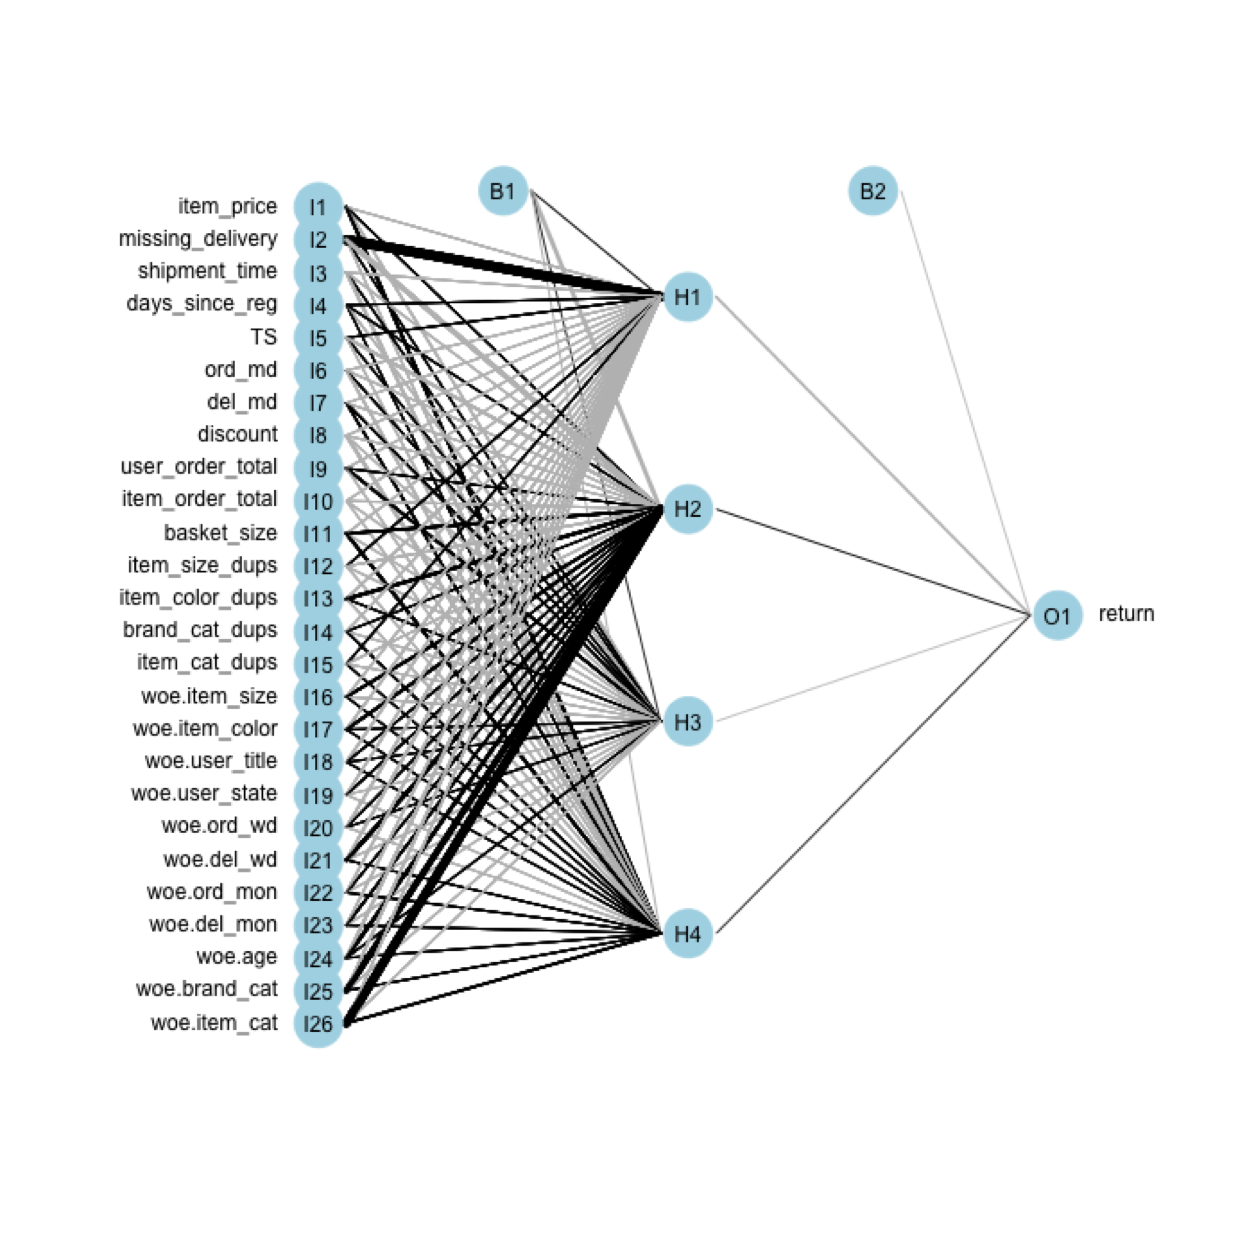
\includegraphics[scale = 0.8]{plot_nn.png}
 	\end{scriptsize}
      \begin{center}
    \caption{Neural Network}  \quantnet {SPLPredictionNeuralNetworks} \url{(goo.gl/Bj5KnJ)}
          \label{fig:nn}
 		\end{center}
  \end{figure}
 
	
	
\thispagestyle{empty}
\begin{figure}[b]
    \begin{scriptsize}
     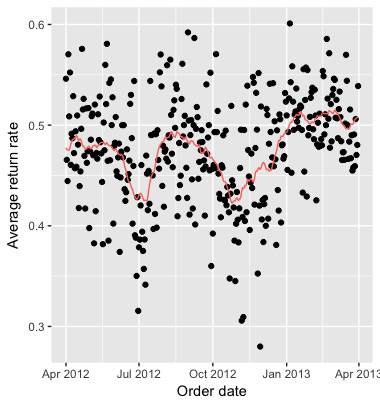
\includegraphics[scale = 0.6]{order_date.png}
 	\end{scriptsize}
      \begin{center}
    \caption{Deterministic Time Series of daily Return rates}
          \label{fig:od}
 		\end{center}
  \end{figure}
		
\thispagestyle{empty}		
\begin{figure}[H]
   \begin{scriptsize}
    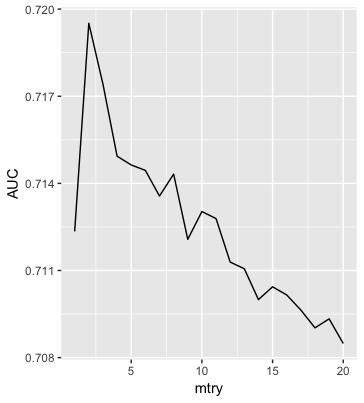
\includegraphics[scale = 0.7]{parameter.png}
 	\end{scriptsize}
      \begin{center}
    \caption{Area under the Curve over allowed Feature Number}
          \label{fig:parameter}
 		\end{center}  
  \end{figure}
\clearpage
\newpage
\section{Tables}	
\thispagestyle{empty}
    \begin{table}[h]
\begin{center}
\begin{tabular}{lc} 
\hline\hline
Classification algorithms & Acronym\\ 
\hline
\noalign{\smallskip}
Neural networks &   NN  \\
Random forest &   RF   \\
Logistic regression &   Logit \\
Decision tree &   DT \\
Regularized regression  &   regLogit  \\
\noalign{\smallskip}
\hline\hline
\end{tabular}
\end{center}
\caption{Prediciton Models}
\label{tab:overview}
\end{table} 
\smallskip
\begin{table}[H]
\centering
\begin{tabular}{llllll}
 &            & \multicolumn{1}{l|}{}                                & \multicolumn{2}{c}{True value}                                              &  \\
 &            & \multicolumn{1}{l|}{}                                & \multicolumn{1}{r}{item kept (0)}    & \multicolumn{1}{r}{item returned (1)} &  \\ \cline{1-5}
 & Prediciton & \multicolumn{1}{l|}{item kept (0) / no intervention} & \multicolumn{1}{r}{0}                & 0.5 * -(3 + 0.1 * itemvalue)          &  \\
 &            & \multicolumn{1}{l|}{item returned (1) / warning}     & \multicolumn{1}{r}{-0.5 * itemvalue} & \multicolumn{1}{r}{0}                 &  \\
 &            &                                                      &                                      &                                       &  \\
 &            &                                                      &                                      &                                       &  \\
 &            &                                                      &                                      &                                       &  \\
 &            &                                                      &                                      &                                       &  \\
 &            &                                                      &                                      &                                       & 
\end{tabular}
\caption{Cost matrix for model assessment.}
\label{tab:cost matrix}
\end{table}
\end{appendices}
\newpage
\bibliographystyle{apacite}
\bibliography{References}

\end{document}
